\begin{center}
\section{Introduction}
\end{center}
\subsection{Theory}
** TODO Combine into one section with litrev \\
% present a history and motivation for the DMP
%Throughout history, scientifically-minded individuals have sought to improve conditions for mankind through manipulation of their environment.  From construction of shelter and wheels up to the development of modern day marvels like nuclear engineering and space flight, human' have developed the ability to produce more, live longer, and have more leisure time through scientific advancement.  For the bulk of history, the majority of scientific development centered around physical observation and experimentation.  From Aristotle's presumption about inertial states of rest to Galileo's assertions about a heliocentric solar system, from Cavendish's gravitational measurements to Young's double-slit experiment with the duality of light, our scientific understanding has developed through measurements and experiments.  Even models crafted entirely out of theory, as with Einstein's theories of relativity, had difficulty taking root until events like Eddington's expedition to Principe, where he was able to detect bending of star light around the gravitational field of the sun during a total solar eclipse.
%
%Unfortunately, along with the march of scientific knowledge, the expense and difficulty of experimentation has similarly increased.  While the nuclear power industry has its roots in Fermi and Szilard's critical pile in Chicago, regulatory bodies can't financially or safely afford to take a ``build and see'' approach with new nuclear power plant designs.  There are some options to help ameliorate this situation.  For instance, a scaled-down facility like the APEX at Oregon State University can be constructed.  Because of the expense in constructing a facility like an AP1000 nuclear power plant, a smaller but hydraulically similar setup like the APEX allows for data collection and analysis with much less expense.  However, even a scaled-down facility can be very expensive to build, leaving a void for a tool that will allow inexpensive calculations to be quickly run a priori to determine the viability of a concept or design.  Computational methods fill this void wonderfully.
This thesis explores the expansion of methods used to bound the \gls{imc} equations used to perform radiative heat transfer simulations.  Along with convection and conduction, radiation  is one of three recognized methods for heat transfer.  Convection and conduction are typically dominant.  As temperature increases or the medium for convection and conduction is removed, however, radiative heat transfer becomes critical in understanding thermal dynamics.  Because of its nonlinear dependent variables, numerical methods are used to solve radiative heat transfer problems.

\subsection{Numerical Modeling}
Historically, the advent of supercomputing gave researchers the ability to turn from very simple models as approximations of real systems to increasingly complex models that more accurately represent real-life systems.  While advances in computational capability offer the potential for more accurate solutions than hand-calculations for difficult problems, these solutions come at a cost.  Traditionally, computations are performed analytically; when this isn't practical, assumptions can be made to simplify the problem so it can still be solved analytically.  When a computer is involved, however, it is almost always necessary to approximate a problem that is continuous in reality as one that is discrete in the numerical model.  While in reality space, time, direction, and energy are often considered continuous in reality, numerical models usually require breaking these dimensions into discrete bins of similar properties \cite{lewis}.

The transition from hand calculations to computational solutions also requires a change in thinking.  Two major schools of thought emerged as scientists embraced the binary-centric properties of computers: stochastic methods, which revolve around using pseudo-random numbers to simulate probabilistic interactions; and deterministic methods, which use characteristic bands of data to represent the problem as a whole.
% TODO flesh this section out more

\subsection{Monte Carlo Methods} \label{montecarlo}
The subset of general numerical methods for particle transport focused on in this work is stochastic methods.  These use computer-generated pseudo-random numbers to probabilistically approach problem solutions.  Primary among general stochastic methods is the Monte Carlo approach, named after the French city on the Mediterranean Sea famous for its casino environment.  The genesis of this method is commonly attributed to Stan Ulam \cite{eckardt}.  Ulam shared his ideas with John von Neumann in 1946 and he in turn began the development of Monte Carlo methods.  In some unpublished remarks captured by Roget Eckhardt, Ulam describes his thought development:
\begin{quote}
The first thoughts and attempts I made to practice [the Monte Carlo Method] were suggested by a question which occurred to me in 1946 as I was convalescing from an illness and playing solitaires. The question was what are the chances that a Canfield solitaire laid out with 52 cards will come out successfully? After spending a lot of time trying to estimate them by pure combinatorial calculations, I wondered whether a more practical method than "abstract thinking" might not be to lay it out say one hundred times and simply observe and count the number of successful plays. This was already possible to envisage with the beginning of the new era of fast computers, and I immediately thought of problems of neutron diffusion and other questions of mathematical physics, and more generally how to change processes described by certain differential equations into an equivalent form interpretable as a succession of random operations. Later [in 1946], I described the idea to John von Neumann, and we began to plan actual calculations. \cite{eckardt}
\end{quote}

As suggested in Ulam's description, some problems are unwieldy to calculate directly.  The Monte Carlo method provides an alternative whereby several ``test'' cases are run and then extrapolated to include the whole problem.  For example, finding the area of black squares on a checkerboard is a simple matter of measuring the length and width of a single black square and multiplying by the number of squares (see Figure \ref{checker}a).  Consider, however, an irregular checkerboard pattern such as in Figure \ref{checker}b).  Finding the area of the black squares would be much more difficult for an irregular orthogonal pattern, let alone a board of irregular shapes of varied sizes.  A Monte Carlo approach to this problem could be tossing down grains of rice one at a time and tallying whether they landed on a white square or black square.  Clearly, if only a few grains of rice are thrown, it is hard to get an accurate representation of the proportion of black area to white area.  If, however, thousands of grains of rice are thrown, a much more accurate picture of proportional area forms.  While it sounds laborious to spend hours throwing rice around, a computer, especially one with parallel processing capabilities, can fly through the rice throwing and tallying in order to return a good estimate of the area quickly.

\begin{figure}[htb]
\centering
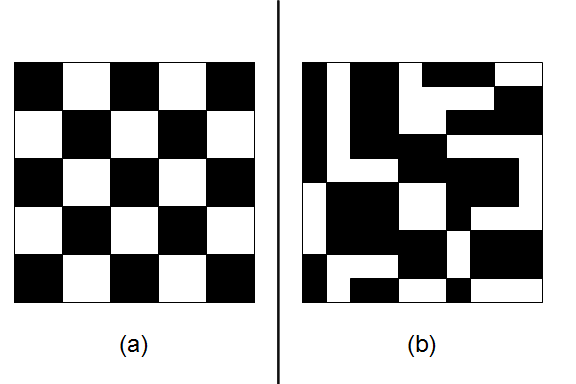
\includegraphics[width=\linewidth]{./graphics/checkers}
\caption{Monte Carlo Checkerboard Example}
\label{checker}
\end{figure}

\subsubsection{Error Quantification in Monte Carlo}

Obviously, this probabilistic approach comes with some level of uncertainty.  This uncertainty is quite different in nature from the uncertainty of direct measurements.  In any numerical method, several sources of error and uncertainty exist, including equation simplification and  discretization errors.  In deterministic methods, errors additionally rise from the choice of discrete angles.  Monte Carlo methods, however, have their own particular source of errors, commonly referred to as variance.

Equation simplification errors originate in the manipulation of complex systems to make them more manageable.  One common manipulation is simplifying the equations to remove or approximate difficult terms.  For example, the outer surface area of a cylinder is the combination of the outside area along the length of the object as well as the circular area on the ends; however, if the length is much larger than the diameter of the cylinder, it may be practical (and introduce minimal errors) to simplify this area and simply use the outside area along the length.  While this error might seem minimal for a particular problem, making such a simplification could introduce unexpectedly large errors for other problems.  Another common manipulation is linearization, wherein a system dependent on the square (or higher power) of a variable can be adjusted to depend only linearly on that variable.  This is common in time-dependent problems, where one method of linearization is to depend largely on previous time steps.  For example, in radiative heat transfer the Planckian blackbody emission function is dependent on temperature raised to the fourth power.  While this creates an extremely unstable problem if treated directly, linearizing makes it possible to rely mostly on the temperature at an old time step, and only linearly on the temperature at the current time.  Of course, this introduces some error, especially if temperature is changing quickly as a function of time.

Discretization errors, on the other hand, are a necessary evil in numerical methods solved computationally.  As previously mentioned, the binary operation of a computer makes it impossible to consider a continuous function; rather, the function must be taken in discrete pieces.  For instance, in evaluating the temperature of a material, one might discretize spatially by assuming the material is made up of small, micrometer cubed volumes.  One might rationalize that if the volumes are small enough, the temperature will be very close to uniform throughout the volume, so it can be approximated as constant for that specific point in time.  This of necessity introduces some level of error; of necessity, though, this error should reduce quickly as the size of the volumes is decreased dramatically.  Similar errors evolve from discretization of time and energy, and, in the case of deterministic methods, angle.

The third major source of error, and perhaps of chief interest in Monte Carlo calculations, is variance.  Variance is inherent in the method of calculating for Monte Carlo.  Imagine solving a problem considering the eventual resting place of a racquetball as it is thrown into a court.  This could be simulated as a particle reflecting off walls until eventually it lost enough energy to be "deposited" somewhere on the floor.  Simply throwing one ball would result in a falacious conclusion, that all racquetballs thrown would end up in the same square as the sample thrown ball.  However, if thousands of balls were thrown into the court and ending positions measured, a much more accurate conclusion about the ending location of a ball is clear.  In Monte Carlo simulations, the precision of a calculation is measured as the inverse of the \emph{variance}.  In general, variance is loosely defined by the number of particles simulated.  In fact, variance is given by the inverse of the root of the particles run, or
\begin{equation}
\sigma^2=\frac{1}{\sqrt{N}},
\end{equation}
where $\sigma^2$ is the variance ($\sigma$ is the \emph{standard deviation}) and $N$ is the number of particle histories.  While variance can become much more complicated if multiple tallies are combined to yield overall solutions, the error introduced by variance in a Monte Carlo simulation is still reduced by increasing the number of particles used in the simulation.

A distinction should be made clear when discussing ``particles'' in Monte Carlo simulations.  It's natural to want to think of Monte Carlo particles as the particle they simulate (whether it be neutrons, photons, or racquetballs).  This is not strictly true, however.  To continue with our example, say you want to throw exactly 100 racquetballs and use Monte Carlo to predict their resting places beforehand.  100 Monte Carlo particles will result in a $1/\sqrt{100}$ variance, or a variance of 0.1, or a standard deviation of just over 0.3.  This translates into a 95\% uncertainty that the balls is within 60\% of the mean!  Chances high that we want much better precision.  We naturally would increase the number of particles run, but can 100 balls be represented by 10,000 Monte Carlo particles?  The answer is typically yes, although converting from particles to neutrons or especially photons may be somewhat complicated.  Regardless, it is important to refrain from thinking of individual Monte Carlo particles as direct representatives of individual photons or neutrons.

\subsection{Radiative Heat Transfer}
One of the more difficult nonlinear problems to solve in particle transport is photon transport in radiative heat transfer.

\subsection{Implicit Monte Carlo Equations}
  Classically we consider three major forms of heat transfer: conduction (ice placed on a metal pan), convection (water flowing past a hot plate), and radiation (the sun warming the earth). Radiative heat is delineated by Planck's description of photon emission from warm bodies and subsequent absorption into background material.  Planckian photon emission can commonly be observed in a material heated until it ``glows red hot.''  As described by the Planckian emission spectrum, all objects emit photons in a spectrum of wavelengths.  Radiative heat transfer is normally insignificant next to convective and conductive heat transfer; however, in relatively high temperatures, this form of heat transfer can be the dominate method.  There are several situations in which radiative heat transfer dominates, including inertial confinement fusion, high-heat thermal hydraulics, and many celestial systems in astrophysics.

The chief difficulty in solving radiative heat transfer problems is the nonlinear dependence on temperature; in fact, the photon emission term relies on the \emph{fourth power} of temperature.  When considered along with the integro-differential nature of most particle transport problems, a truly difficult set of coupled equations emerge.  Fortunately, through the inspiration of J.A. Fleck and J.D. Cummings, the radiative heat transfer equations can be reformed to a form that is more easily solved through numerical methods.  It is important to note that these reformed equations, while called the \gls{imc} equations, can be solved equally well with deterministic or Monte Carlo methods.  As with any approximation that simplifies or linearizes a system, though, the \gls{imc} equations come with their own concerns; in particular, violations of a weak maximum principle.
 


\subsection{Discrete Maximum Principle}
As expected, Fleck and Cummings found some boundedness concerns with the \gls{imc} equations.  ``Boundedness'' refers to the ability of the code to return results that are physically viable.  For instance, in a problem consisting of a straight section of pipe with no leaks or sources, the mass flux entering the section must be the same as that leaving.  The boundedness problem Fleck and Cummings encountered involves holding one boundary of a material at a given hot temperature and allowing the other end to be vacuum.  For a given choice of time step size, Fleck and Cummings found a spatial step size that caused an unphysical spike of temperature in the material \emph{greater} than the hot boundary temperature.  Restated, this erroneous result suggests that putting a cold material up against a hot one results in a spiked temperature in the cold material higher than the hot one.  Clearly this is unbounded, and an artifact of the numerical method.  This undesirable result of using the \gls{imc} equations led researchers to seek out equations to satisfy a maximum principle, or a set of equations that determine the range of time and space steps that are guaranteed to return physical results.

In the realm of partial differential equations, a maximum principle usually applies to parabolic or elliptic equations, and maximum principles in general require maximum conditions to exist on the boundary of the problem.  A wide variety of maximum principles exist.  One, the \emph{strong} maximum principle, declares that if a function reaches its maximum on the interior of the problem, it must be constant throughout.  The maximum principle we concern ourselves with, however, is that simplest of weak maximum principles: given a hot boundary condition, no interior temperatures can be greater than the hot condition temperature.

Fleck and Cummings first acknowledged the violation of the maximum principle in their landmark paper on the \gls{imc} equations, saying
\begin{quote}
The $ct=6$ cm curve is inaccurate near the source ... although the
remainder of the curve does not look bad. \cite{FleckCumm}
\end{quote}
This is in reference to their choice of time step size for a particular problem (see Literature Review section of this thesis for more details).

Also described in further depth in the Literature Review section of this thesis, Larsen and Mercier approached this maximum principle by taking time as discretized and space as continuous.  After significant derivations, an inequality is devised to govern the time step such that the solution will not violate the weak maximum principle.  In light of future work, these can be referred to as the \gls{cmp} equations.  Unfortunately, Larsen and Mercier found that their estimation of time step restriction was severe.  In addition, they compared the \gls{cmp} limits to experimental data and found a much larger time step could be used most of the time than was predicted.  Interestingly, there also appeared to be a relationship between spatial step and the maximum principle, which lead to the next and most recent development in the search for bounding the \gls{imc} equations.

Noting the association of both time and step size with violations of the weak maximum principle, Wollaber, Larsen, and Densmore derived a new set of governing equations, referred to as the \gls{dmp} equations.  While this initial \gls{dmp} was derived with some simplifying assumptions and implemented pseudo-analytically for a particular problem, this \gls{dmp} much more accurately predicted time step limits that match experimental data.

The work of this thesis is to remove some of the assumptions made in the \gls{dmp} and implement it rigorously into an existing radiative heat transfer code and demonstrate fidelity in multiple dimensions, non-equilibrium initial conditions, and problems other than the Marshak wave.